\documentclass{fancyslides}
%% Presentation was created using:
%% Fancyslides class, by Pawel Lupkowski
%% http://www.staff.amu.edu.pl/~p_lup/?page_id=1057
%%
%\usepackage{fontspec}

%% Beamer settings (do not change)
\usetheme{default} 
\setbeamertemplate{navigation symbols}{} %no navigation symbols
\setbeamercolor{structure}{fg=\yourowntexcol} 
\setbeamercolor{normal text}{fg=\yourowntexcol} 

%%
%% Extra package
%%

%% Aspect ratio
\newcommand{\aspectW}{40}
\newcommand{\aspectH}{18}
\usepackage[orientation=landscape,size=custom,width=\aspectW,height=\aspectH,scale=0.5,debug]{beamerposter}
\usepackage{comment}

%%
%% GRID & STYLE
%%
\usepackage{tikz}
%\usetikzlibrary{arrows,positioning}
\usetikzlibrary{arrows, decorations.markings,positioning, decorations.pathreplacing}
%% MY STYLE AND COMMAND FOR TIKZ
\tikzset{tick/.style={below=3pt}}

%%
%% Function to call the grid
%% Usage:
%% \showTheGrid{1} TRUN ON
%% \showTheGrid{0} TRUN OFF
\newcommand{\showTheGrid}[1]{
    \draw[step=1cm,gray,very thin, opacity=#1] (0,0) grid (\aspectW,\aspectH);
    \foreach \x in {1,...,\the\numexpr\aspectW-1} {
%%		\draw [blue, opacity=#1] (\x,\aspectH/2) -- (\x,\aspectH/2) node[below] {\huge{\x}};
    \ifodd\x\relax
		\draw [blue, opacity=#1] (\x,\aspectH/2) -- (\x,\aspectH/2) node[below] {\huge{\x}};
		\else
	\fi }
    \foreach \y in {1,...,\the\numexpr\aspectH-1} {
%		\draw [red, opacity=#1] (\aspectW/2,\y) -- (\aspectW/2,\y) node[right] {\huge{\y}};
    \ifodd\y\relax
		\draw [red, opacity=#1] (\aspectW/2, \y) -- (\aspectW/2, \y) node[right] {\huge{\y}};
		\else
	\fi }
		}

%% Multilanguage support
%% every time one must be activated and the other deactivated
\includecomment{reversedOn}
\excludecomment{reversedOff}

%%%%%%%%%%%%%%%%%%%%%%%%%
%%% CUSTOMISATIONS %%%%%%
%%%%%%%%%%%%%%%%%%%%%%%%%

% THE FOLLOWING COLOURS ARE PREDEFINED IN THE CLASS
%bi -- WHITE
%cz -- BLACK
%sz -- GRAY
%nieb -- BLUE
%ziel -- GREEN
%pom -- ORANGE
%% YOU CAN DEFINE YOUR OWN COLOUR TO USE HERE. SEE MAN.PDF


%%%% SLIDE ELEMENTS
\newcommand{\structureopacity}{0.75} %opacity for the structure elements (boxes and dots)
\newcommand{\strcolor}{nieb} %elements colour (predefined nieb; pom; ziel)

%%%% TEXT COLOUR
\newcommand{\yourowntexcol}{cz}

%% COMMAND TO FIX THE LOGO POSITION (x,y) in cm
\usepackage[absolute,overlay]{textpos}
\setlength{\TPHorizModule}{1cm}
\setlength{\TPVertModule}{1cm}
\newcommand{\MyLogo}{%
   \begin{textblock}{14}(7.0,3.0)
      
\includegraphics[height=6cm,angle=0]{figures/MyLogo}
   \end{textblock}
   }

%%%%%%%%%%%%%%%%%%%%%%%%%
%%% TITLE SLIDE DATA %%%%
%%%%%%%%%%%%%%%%%%%%%%%%%
\newcommand{\titlephrase}{Banner for "How to merge odd and even pages together in a PDF with \LaTeX{}"}
\newcommand{\name}{Nicola Rainiero}
\newcommand{\affil}{\href{http://rainnic.altervista.org}{rainnic.altervista.org}}
\newcommand{\email}{\href{mailto:rainnic@altervista.org}{rainnic@altervista.org}}
\newcommand{\firm}{Rainnic in the clouds}
\title{\titlephrase}
\newcommand{\keyWords}{LaTeX, online, Overleaf, split, crop}

%%
%% URL ADVANCED
%%
\usepackage{hyperref}
\hypersetup{
	pdftitle={\@title},
	pdfsubject={\firm},
	pdfauthor={\name},
	pdfkeywords={\keyWords},
	%pdfpagemode=FullScreen, % once opened it goes in fullscreen mode
	%citecolor=black,
	%filecolor=black,
	%linkcolor=black,
	%urlcolor=black
}

\begin{document}
%\fontspec[Ligatures={TeX}]{Lato} %% SETS THE FONT FOR THE PRESENTATION

\fbckg{figures/background}
\begin{frame}
%\MyLogo
 \makebox[\textwidth][c]{\begin{tikzpicture}
    \showTheGrid{0}

%\shadedraw[left color=white, right color=gray, draw=white] (19.5,0) rectangle (40,16.0);

\shadedraw[bottom color=white, top color=gray!80!teal, draw=white] (0,0) rectangle (\aspectW,\aspectH);

\node[](A) at (4,13.5) {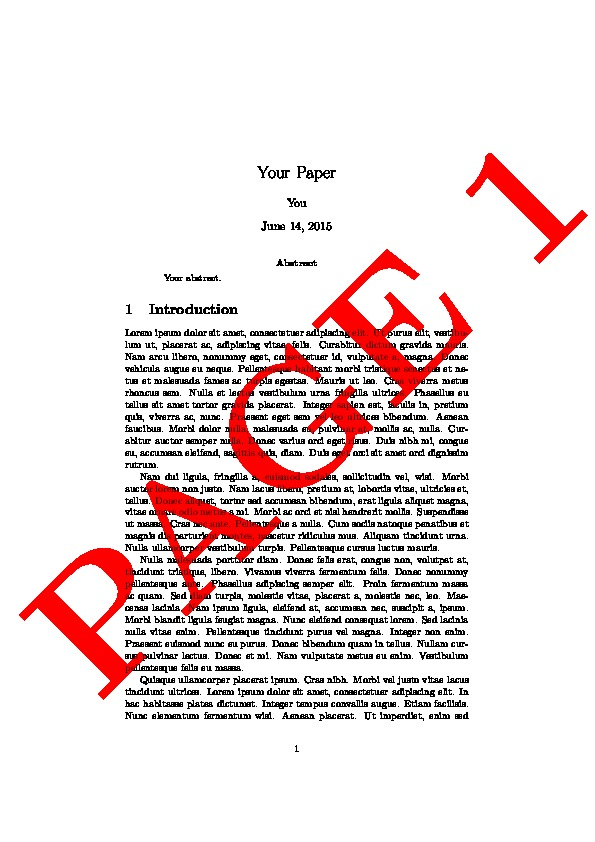
\includegraphics[height=0.3\textheight]{figures/page_0}};

\node[](C) at (8,13.5) {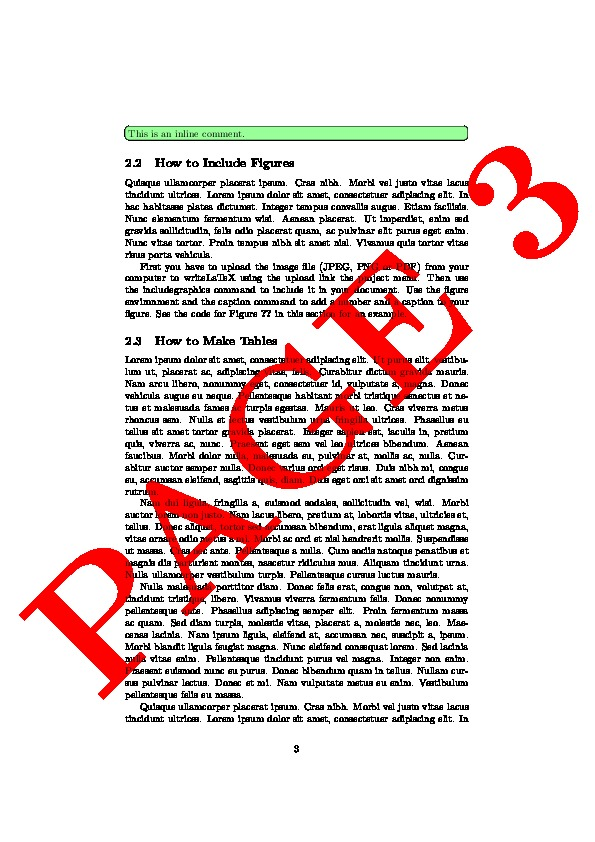
\includegraphics[height=0.3\textheight]{figures/page_2}};

\node[](E) at (12,13.5) {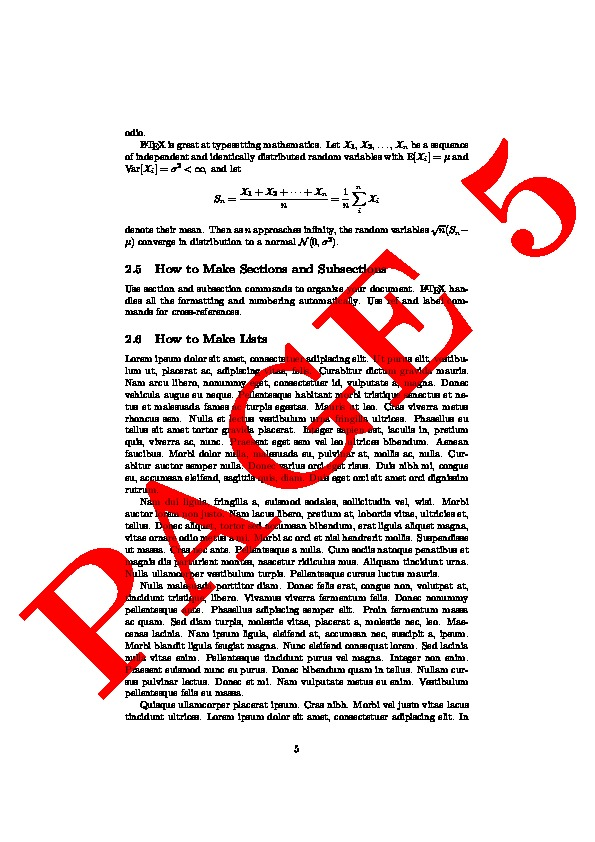
\includegraphics[height=0.3\textheight]{figures/page_4}};

\draw[thick, red!80!olive, decoration={brace,mirror,amplitude=1cm}, decorate,line width=5] (2,10.5) -- (14,10.5) node[midway, below=1.0cm, text opacity=0.95, align=center, sloped]{\Huge{ODD PAGES}};

%% Reversed ON
\node[](F) at (4,5.5) {
\includegraphics[height=0.3\textheight]{figures/page_5}};

\node[](D) at (8,5.5) {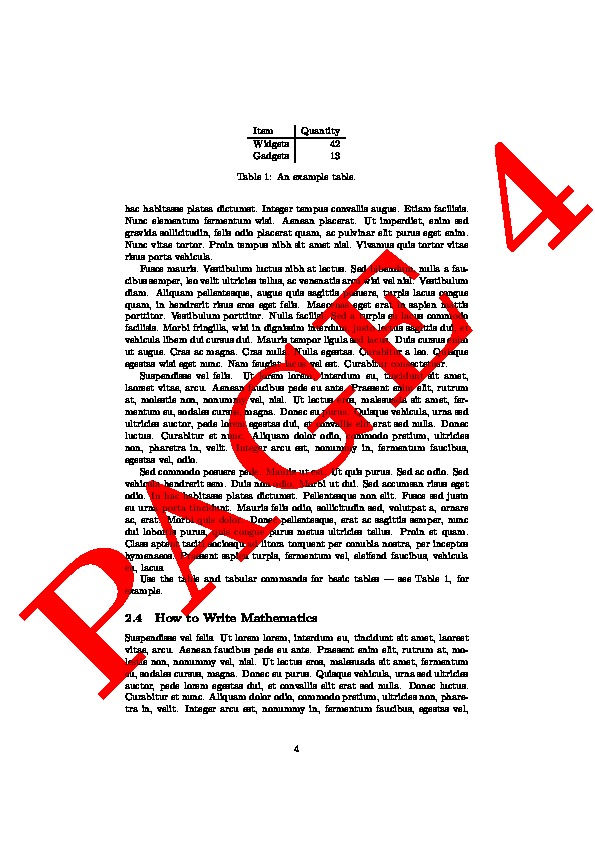
\includegraphics[height=0.3\textheight]{figures/page_3}};

\node[](B) at (12,5.5) {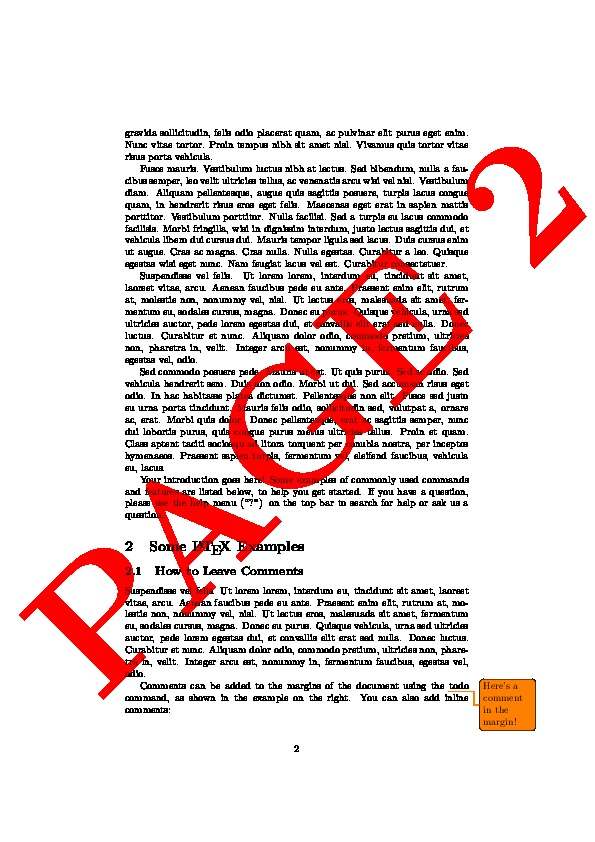
\includegraphics[height=0.3\textheight]{figures/page_1}};

\draw[thick, red!80!olive, decoration={brace,mirror,amplitude=1cm}, decorate,line width=5] (2,2.5) -- (14,2.5) node[midway, below=1.0cm, text opacity=0.95, align=center, sloped]{\Huge{EVEN PAGES (REVERSED)}};
%% Reversed ON

%% Reversed OFF
%\node[](F) at (4,5.5) {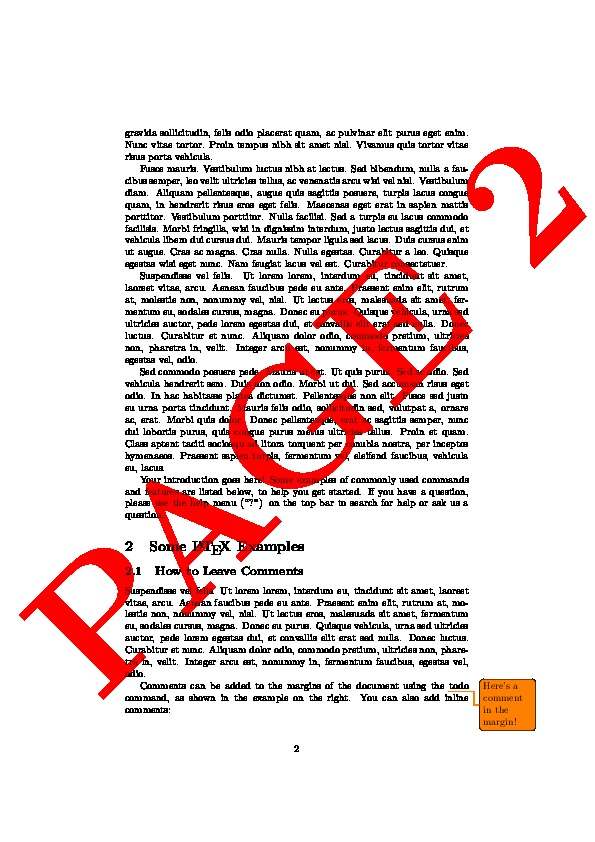
\includegraphics[height=0.3\textheight]{figures/page_1}};

%\node[](D) at (8,5.5) {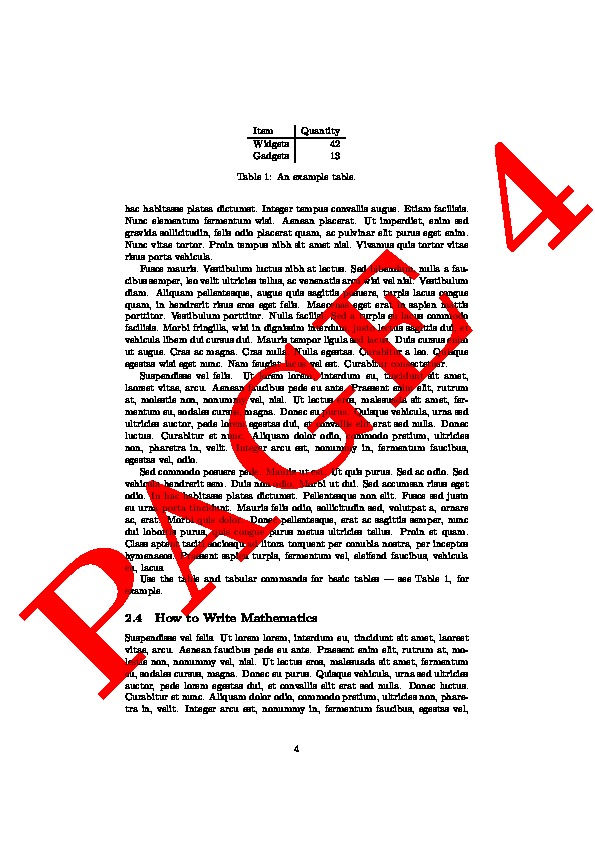
\includegraphics[height=0.3\textheight]{figures/page_3}};

%\node[](B) at (12,5.5) {
\includegraphics[height=0.3\textheight]{figures/page_5}};

%\draw[thick, red!80!olive, decoration={brace,mirror,amplitude=1cm}, decorate,line width=5] (2,2.5) -- (14,2.5) node[midway, below=1.0cm, text opacity=0.95, align=center, sloped]{\Huge{EVEN PAGES}};
%% Reversed OFF

\draw[*-triangle 45, line width=5] (14,9) -- (24.5,9) node [midway, text opacity=0.95, draw=gray, ultra thin, rounded corners=.25ex, fill=gray!20,text width=5cm, align=center,sloped] {\huge{\LaTeX{}}};

\node[] at (27,11.75) {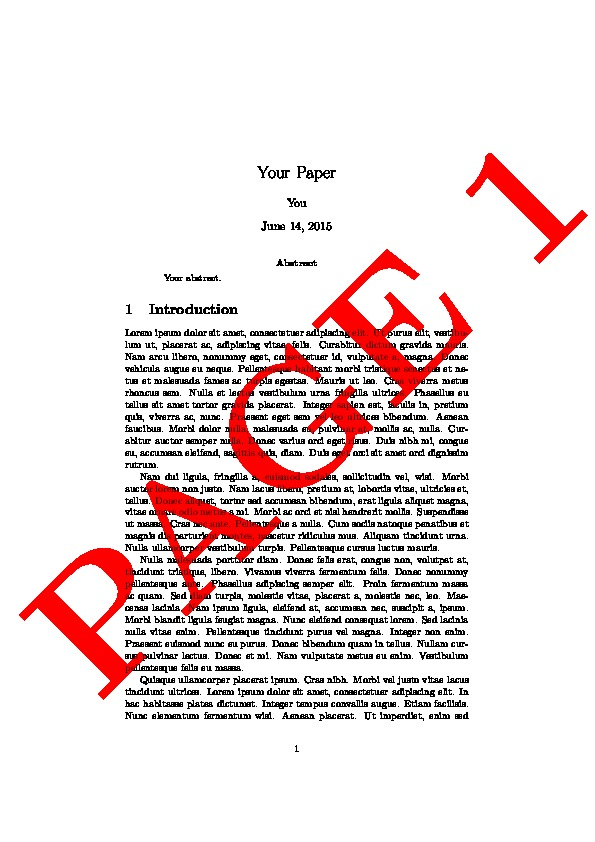
\includegraphics[height=0.3\textheight]{figures/page_0}};

\node[] at (31,11.75) {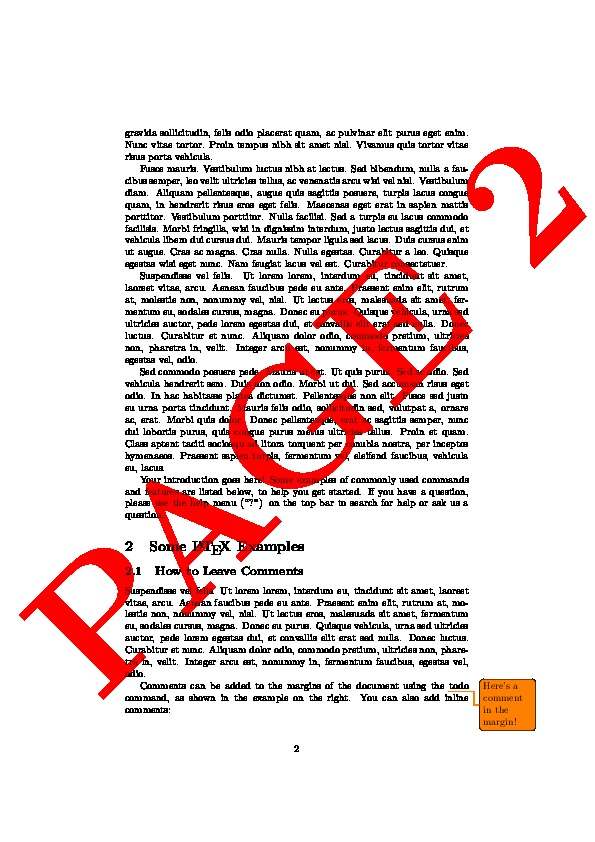
\includegraphics[height=0.3\textheight]{figures/page_1}};

\node[] at (35,11.75) {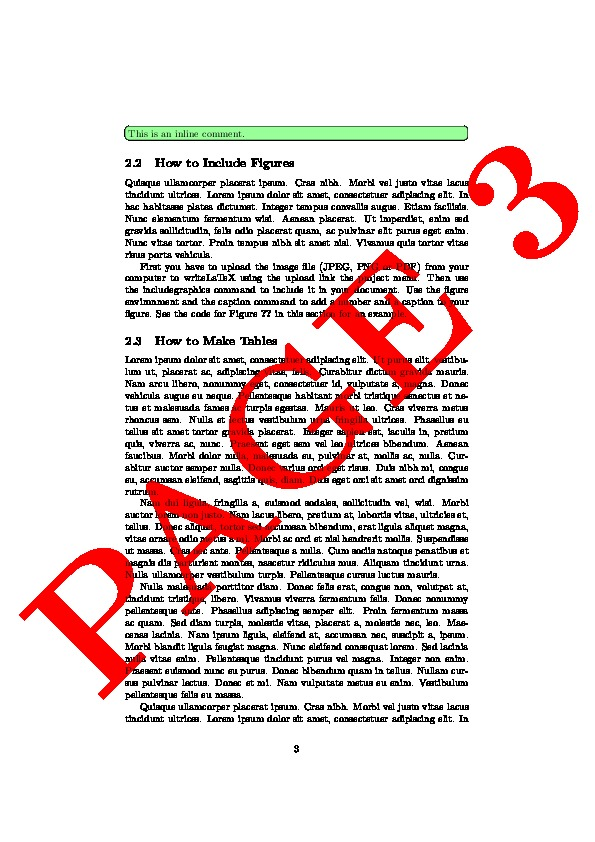
\includegraphics[height=0.3\textheight]{figures/page_2}};

\node[] at (27,6.25) {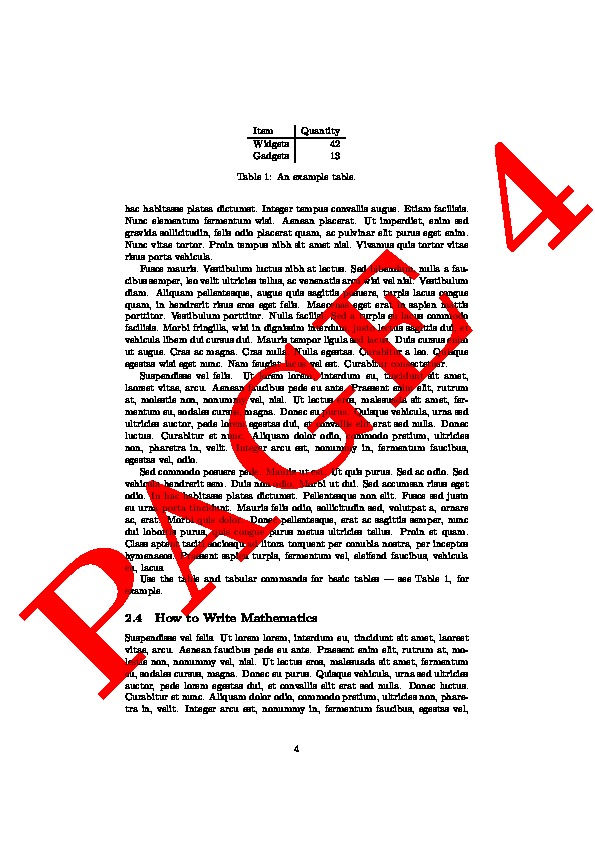
\includegraphics[height=0.3\textheight]{figures/page_3}};

\node[] at (31,6.25) {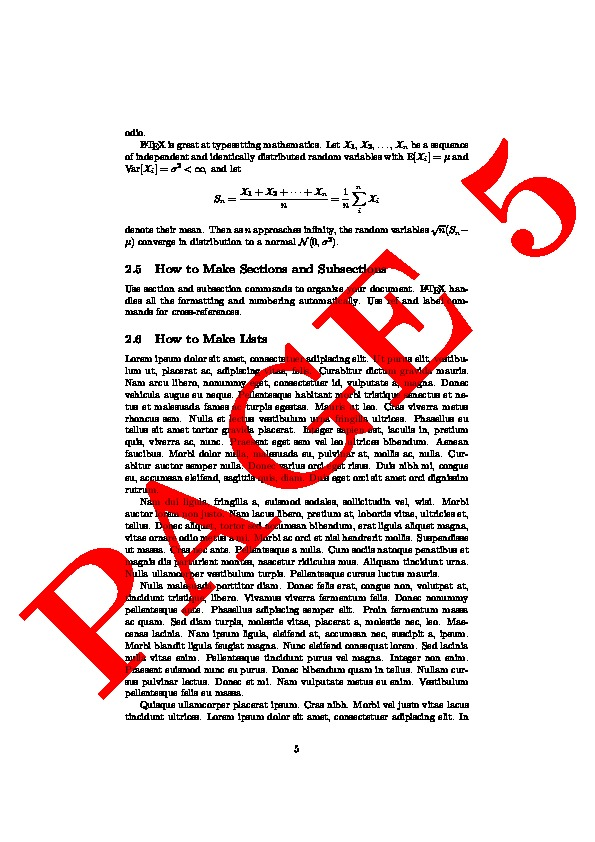
\includegraphics[height=0.3\textheight]{figures/page_4}};

\node[] at (35,6.25) {
\includegraphics[height=0.3\textheight]{figures/page_5}};

\draw[thick, red!80!olive, decoration={brace,mirror,amplitude=1cm}, decorate,line width=5] (25,2.5) -- (37,2.5) node[midway, below=1.0cm, text opacity=0.95, align=center, sloped]{\Huge{MERGED PDF}};

\node[opacity=0.9] at (19,5.0) {
\includegraphics[height=0.3\textheight]{figures/pdf_icon.png}};

  \end{tikzpicture}
  }
\end{frame}

\end{document}